\chapter{Sprint documents}

\begin{figure}[h!]
	\centering
	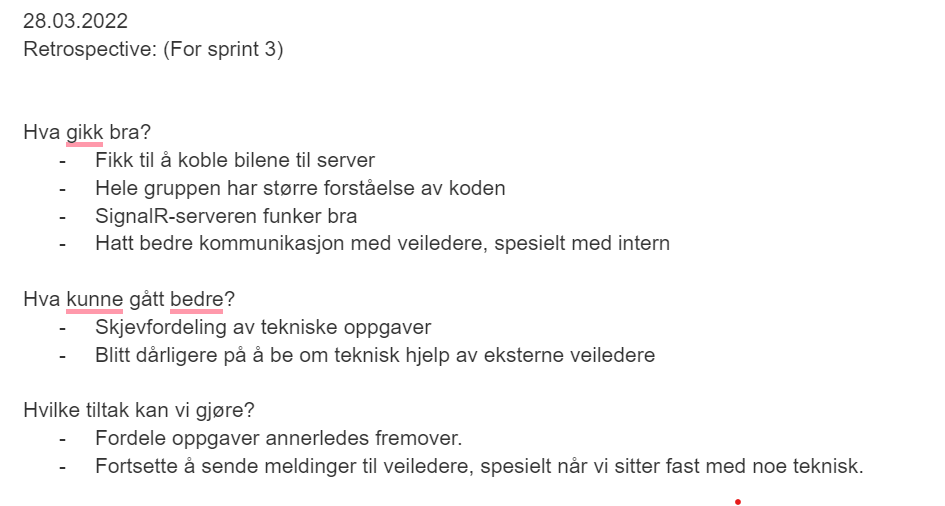
\includegraphics[width=1\linewidth]{figures/sprint_retroperspective}
	\caption[Sprint retroperspective]{A snapshot of a sprint retroperspective meeting from our log. There are three sections: What went well? What could have gone better? And what can we do for next time?}
	\label{fig:sprintretroperspective}
\end{figure}

\begin{figure}[h!]
	\centering
	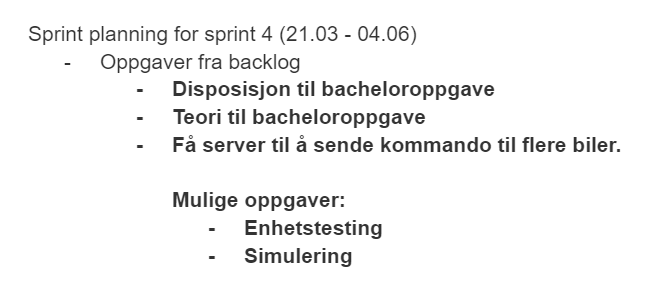
\includegraphics[width=1\linewidth]{figures/sprint_planning}
	\caption[Sprint planning]{A snapshot of a sprint planning meeting from our log. The upper section contains the tasks we are going to do from the backlog. The section under contains possible but not necessary tasks.}
	\label{fig:sprintplanning}
\end{figure}

\begin{figure}[h!]
	\centering
	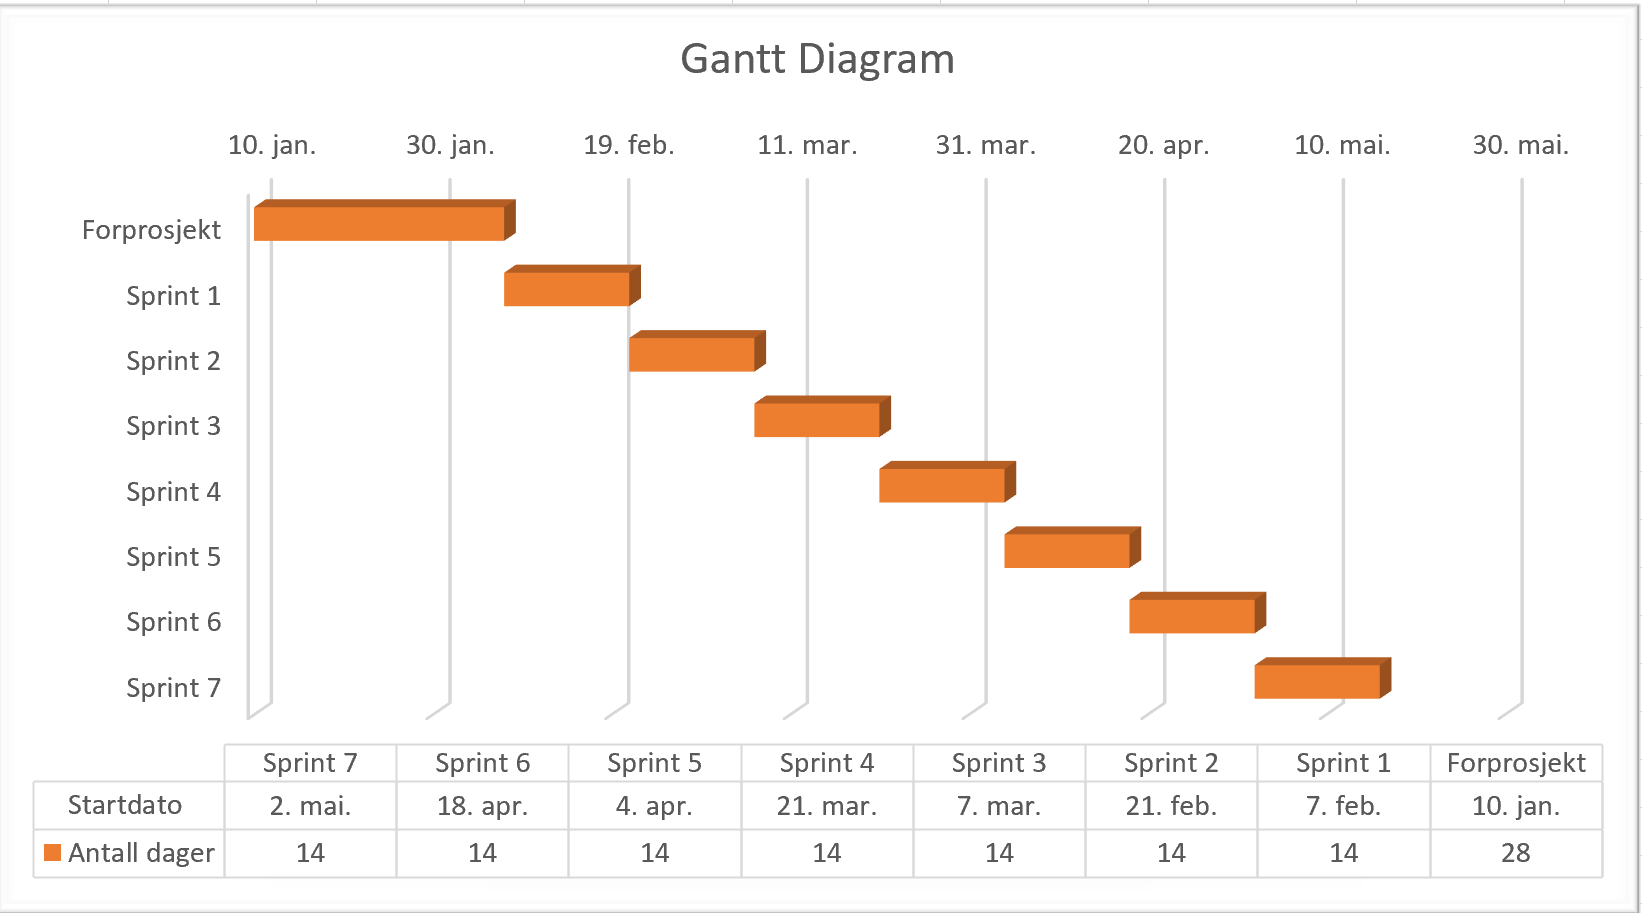
\includegraphics[width=1\linewidth]{figures/gantt}
	\caption[Sprint planning]{A Gantt diagram visualizing the duration of each sprint. Each sprint lasted two weeks, while the pre-project phase lasted four weeks.}
	\label{fig:gantt}
\end{figure}